\documentclass[tikz,border=2mm]{standalone}
\usepackage{amssymb}
\usepackage{tikz}
\usetikzlibrary{positioning,calc}

\begin{document}

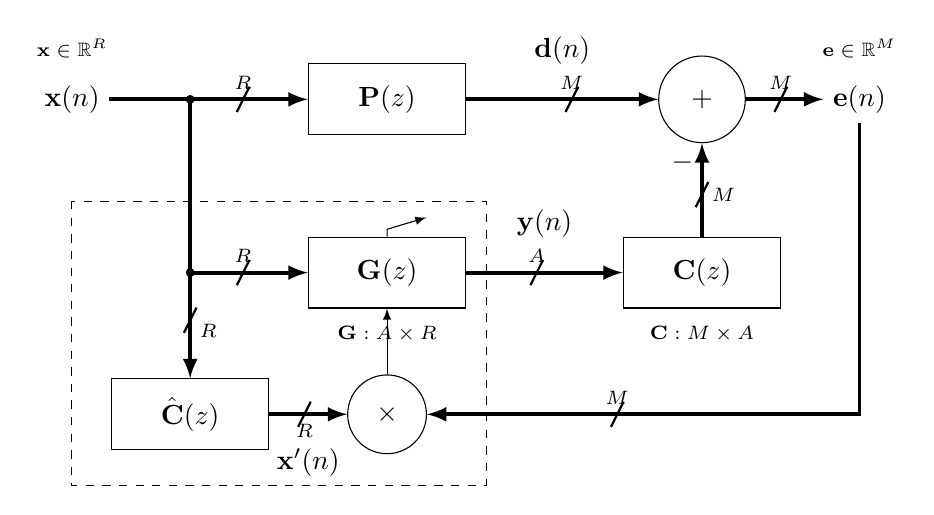
\begin{tikzpicture}[
    block/.style={draw, rectangle, minimum width=20mm, minimum height=9mm},
    sum/.style={draw, circle, minimum size=11mm},
    mult/.style={draw, circle, minimum size=10mm},
    bus/.style={line width=1.4pt},
    busarrow/.style={->, line width=1.4pt},
    thinarr/.style={->},
    >=latex
]

% Helper macro for bus marks
\newcommand{\busmark}[3]{%
    \draw[line width=0.8pt] ($(#1)!#3!(#2)+(-0.08,-0.16)$) --
                           ($(#1)!#3!(#2)+(0.08,0.16)$);
}

\newcommand{\buslabel}[4]{%
    \node at ($(#1)!#3!(#2)+#4$) {\scriptsize $#3$};
}

% Main nodes
\node (x) at (0,0) {$\mathbf{x}(n)$};
\node[block] (P) at (4.0,0) {$\mathbf{P}(z)$};
\node[sum] (sum) at (8,0) {$+$};
\node (e) at (10,0) {$\mathbf{e}(n)$};

\node[block] (G) at (4.0,-2.2) {$\mathbf{G}(z)$};
\node[block] (C) at (8,-2.2) {$\mathbf{C}(z)$};

\node[block] (Chat) at (1.5,-4.0) {$\hat{\mathbf{C}}(z)$};
\node[mult] (mul) at (4,-4.0) {$\times$};

% Helper coordinates
\coordinate (xsplit) at (1.5,0);
\coordinate (xmid) at (1.5,-2.2);
\coordinate (xlow) at (1.5,-2.2);
\coordinate (efb1) at (8.9,-4.0);
\coordinate (upd) at (4.0,-1.65);
\coordinate (updend) at (4.5,-1.5);

% Reference input and split
\draw[bus] (x) -- (xsplit);
\fill (xsplit) circle (1.6pt);

\draw[busarrow] (xsplit) -- (P.west);
\draw[bus] (xsplit) -- (xmid);
\draw[busarrow] (xmid) -- (G.west);
\draw[busarrow] (xlow) -- (Chat.north);

\fill (xlow) circle (1.6pt);

% Primary path
\draw[busarrow] (P) -- node[above, yshift=3mm] {$\mathbf{d}(n)$} (sum);

% Secondary path
\draw[busarrow] (G) -- node[above, yshift=3mm] {$\mathbf{y}(n)$} (C);
\draw[busarrow] (C.north) -- (sum.south);

% Error output and feedback
\draw[busarrow] (sum) -- (e);
\draw[bus] (e) |- (efb1);
\draw[busarrow] (efb1) -- (mul.east);

% Filtered-x branch
\draw[busarrow] (Chat.east) -- node[below, yshift=-3mm] {$\mathbf{x}'(n)$} (mul.west);

% Adaptation update
\draw[thinarr] (mul.north) -- (G.south);
\draw[thinarr] (G.north) -- (upd) -- (updend);

% Minus sign outside summing circle
\node at ($(sum.south)+(-0.25,-0.25)$) {$-$};

% Bus marks and labels
\draw[line width=0.8pt] ($(xsplit)!0.45!(P.west)+(-0.08,-0.16)$) --
                       ($(xsplit)!0.45!(P.west)+(0.08,0.16)$);
\node[above] at ($(xsplit)!0.45!(P.west)$) {\scriptsize $R$};

\draw[line width=0.8pt] ($(xmid)!0.45!(G.west)+(-0.08,-0.16)$) --
                       ($(xmid)!0.45!(G.west)+(0.08,0.16)$);
\node[above] at ($(xmid)!0.45!(G.west)$) {\scriptsize $R$};

\draw[line width=0.8pt] ($(xlow)!0.45!(Chat.north)+(-0.08,-0.16)$) --
                       ($(xlow)!0.45!(Chat.north)+(0.08,0.16)$);
\node[right] at ($(xlow)!0.55!(Chat.north)$) {\scriptsize $R$};

\draw[line width=0.8pt] ($(G.east)!0.45!(C.west)+(-0.08,-0.16)$) --
                       ($(G.east)!0.45!(C.west)+(0.08,0.16)$);
\node[above] at ($(G.east)!0.45!(C.west)$) {\scriptsize $A$};

\draw[line width=0.8pt] ($(P.east)!0.55!(sum.west)+(-0.08,-0.16)$) --
                       ($(P.east)!0.55!(sum.west)+(0.08,0.16)$);
\node[above] at ($(P.east)!0.55!(sum.west)$) {\scriptsize $M$};

\draw[line width=0.8pt] ($(C.north)!0.45!(sum.south)+(-0.08,-0.16)$) --
                       ($(C.north)!0.45!(sum.south)+(0.08,0.16)$);
\node[right] at ($(C.north)!0.45!(sum.south)$) {\scriptsize $M$};

\draw[line width=0.8pt] ($(sum.east)!0.45!(e.west)+(-0.08,-0.16)$) --
                       ($(sum.east)!0.45!(e.west)+(0.08,0.16)$);
\node[above] at ($(sum.east)!0.45!(e.west)$) {\scriptsize $M$};

\draw[line width=0.8pt] ($(efb1)!0.45!(mul.east)+(-0.08,-0.16)$) --
                       ($(efb1)!0.45!(mul.east)+(0.08,0.16)$);
\node[above] at ($(efb1)!0.45!(mul.east)$) {\scriptsize $M$};

\draw[line width=0.8pt] ($(Chat.east)!0.45!(mul.west)+(-0.08,-0.16)$) --
                       ($(Chat.east)!0.45!(mul.west)+(0.08,0.16)$);
\node[below] at ($(Chat.east)!0.45!(mul.west)$) {\scriptsize $R$};

% Dashed adaptive block
\draw[dashed]
    ($(Chat.north west)+(-0.5,2.25)$)
    rectangle
    ($(mul.south east)+(0.9,-0.55)$);

% Dimensions
\node[above=1mm of x] {\scriptsize $\mathbf{x}\in\mathbb{R}^{R}$};
\node[below=1mm of G] {\scriptsize $\mathbf{G}: A\times R$};
\node[below=1mm of C] {\scriptsize $\mathbf{C}: M\times A$};
\node[above=1mm of e] {\scriptsize $\mathbf{e}\in\mathbb{R}^{M}$};

\end{tikzpicture}

\end{document}